\documentclass[12pt,letterpaper]{article}
\usepackage[UTF8]{inputenc}
\usepackage[spanish]{babel}
\usepackage{times}
\usepackage{graphicx}
\usepackage{amsmath}
\usepackage{amsfonts}
\usepackage{amssymb}
\usepackage[left=2cm,right=2cm,top=2cm,bottom=2cm]{geometry}
\date{}
\begin{document}
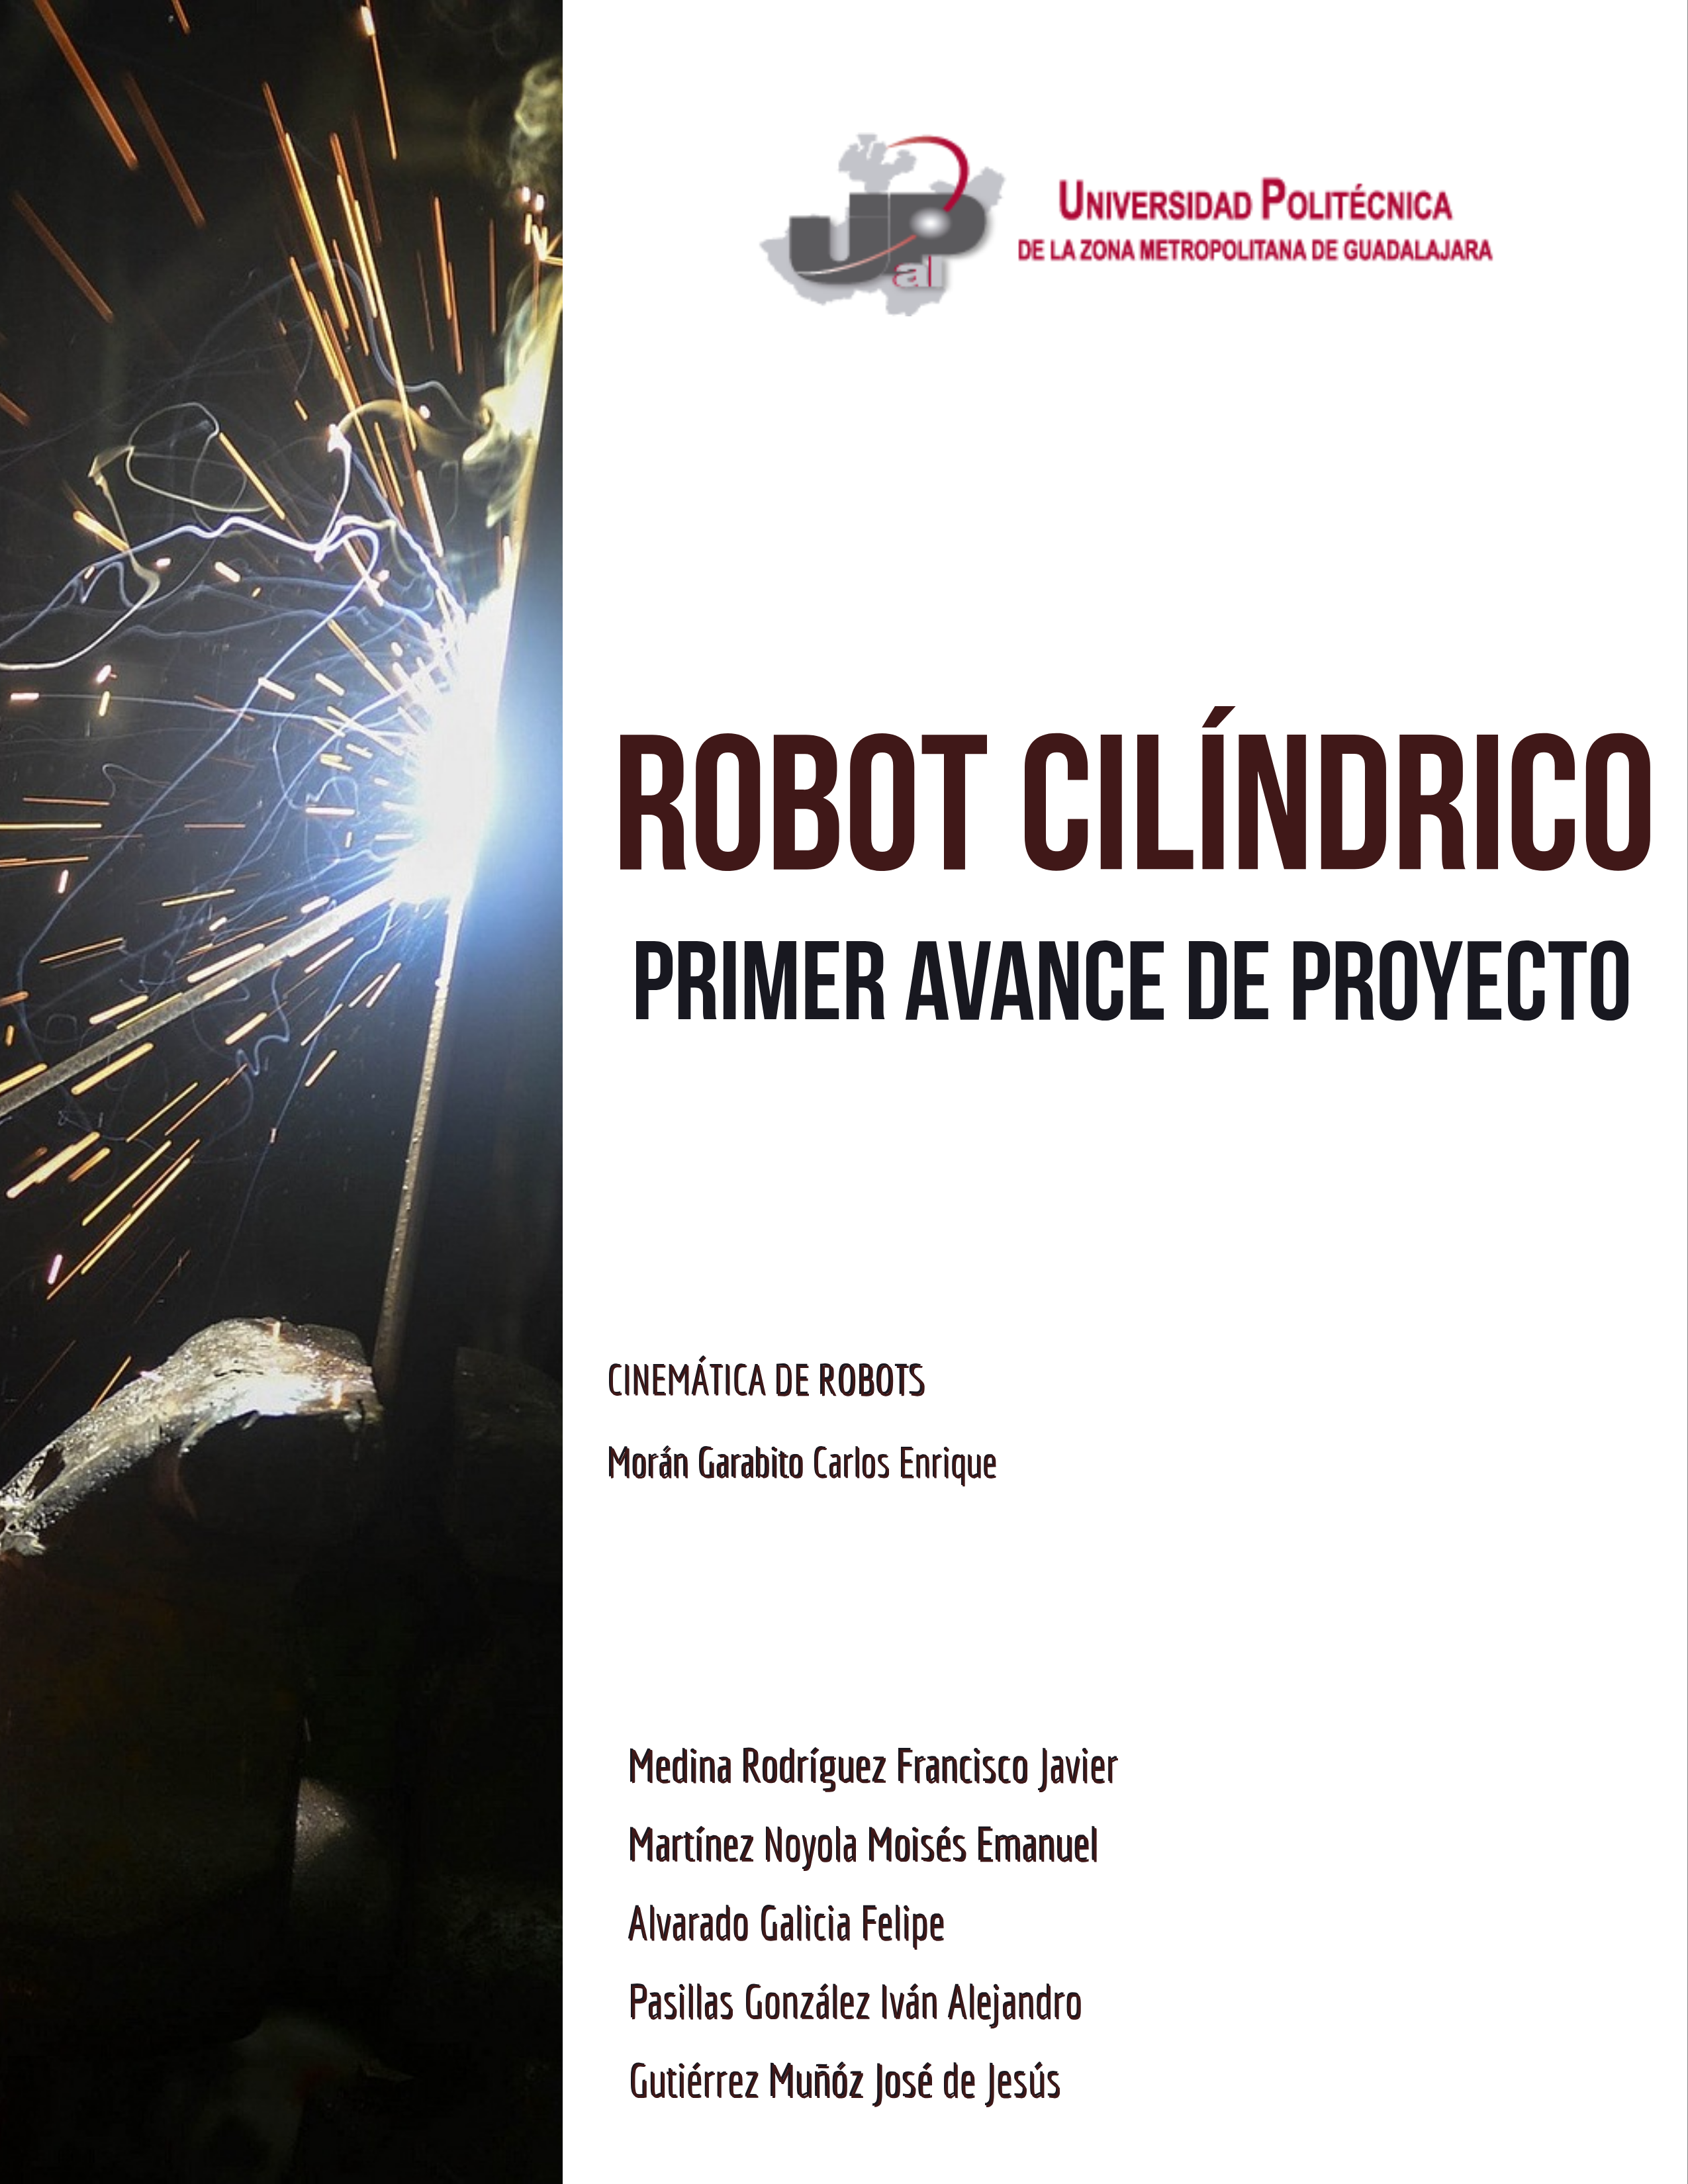
\includegraphics[scale=.2]{imagenes/Portada.png} \\\\
\section{indice}
$$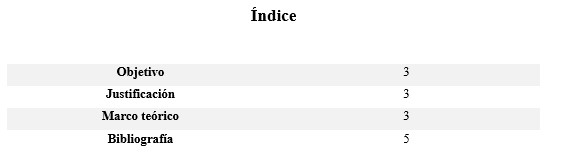
\includegraphics[scale=1]{imagenes/Indice.jpg}$$ \\\\\\\\\\\\\\\\\\\\\\\\\\\\\\\\\\\\\\\\\\\\\\\\\\\\\\\\\\\\\\\\\\\\\\\\
\section{Objetivo}
Construir un robot de tipo cilíndrico, capaz de realizar cordones de soldadura de 5cm en acero, contando con 3 grados de libertad y con dimensiones totales de 50 cm de largo x 30 cm de alto.
\section{Justificacion}
La exigencia de la construcción de un robot para el último ciclo de formación en la ingeniería Mecatrónica nos ha orillado a elegir este proyecto. Con la experiencia en el área de soldadura y herrería de dos integrantes del equipo hemos decidido construir este robot no para fines industriales, sino para uso del taller y como apoyo para el trabajador.
\section{Marco teorico}
¿Qué es un robot industrial?\\

Primero, y de acuerdo con la Asociación de Industrias de Robótica (RIA, Robotic Industry Association), un robot industrial es “un manipulador multifuncional reprogramable, capaz de mover materias, piezas, herramientas, o dispositivos especiales, según trayectorias variables, programadas para realizar tareas diversas.\\O, en otras palabras, una máquina o mecanismo articulado entre sí, el cual tiene 3 distintivos esenciales:
\begin{itemize}
\item Es internacional
\item Puede ser controlado por un operador humano o dispositivo logico
\item Es reprogramable\\
\end{itemize}
Y todo sin hacer modificaciones físicas al robot pues está diseñado, justamente, para realizar tareas variadas y cíclicas que pueden adaptarse.
\subsection{¿Cómo se conforma un robot industrial?}
Además de estas características que definen a los robots industriales, usted también podrá observar que los robots industriales se componen de una estructura parecida, la cual tiene 4 componentes esenciales:
\begin{itemize}
\item •	Tienen un brazo mecánico con capacidad de manipulación, el cual puede ser controlado.
\item •	Se componen de elementos estructurales rígidos, llamados eslabones o enlaces.
\item •	Estos son conectados por articulaciones, las cuales pueden ser lineales o rotatorias.
\item •	Terminan en puntos terminales “manipuladores” los cuales pueden ser pinzas o herramientas.
\end{itemize}
\section{Robot Cilíndrico}
El robot tiene al menos una junta giratoria en la base y al menos una junta prismática para conectar los enlaces. La junta rotativa utiliza un movimiento de rotación a lo largo del eje de la junta, mientras que la junta prismática se mueve en un movimiento lineal. Los robots cilíndricos operan dentro de un sobre de trabajo de forma cilíndrica.
Usado en operaciones de traslado de materiales, ensamblaje, manipulación de máquinas y herramientas, soldadura por punto y manipulación en máquinas de función a presión.
$$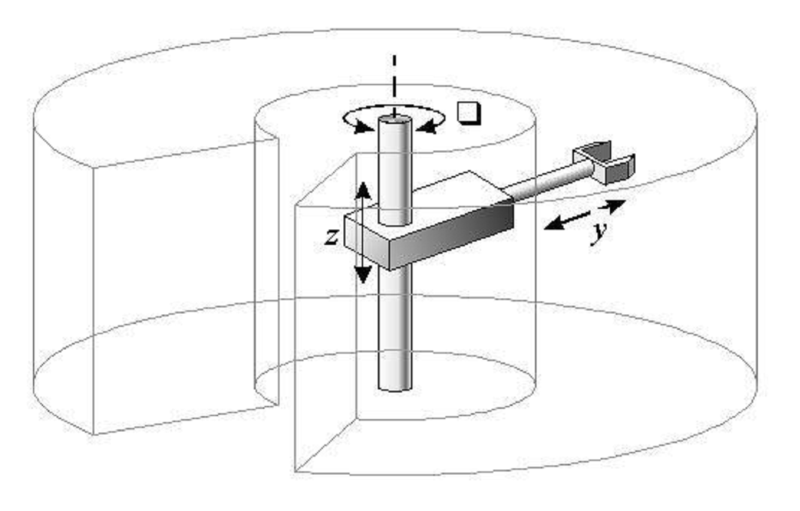
\includegraphics[scale=.7]{imagenes/Imagen.png}$$
\section{Bibliografias}
https://sites.google.com/site/proyectosroboticos/cinematica-inversa-i/brazo-cilindrico\\
https://www.bfmx.com/tipos-de-robots-industriales-mas-utilizados/
\end{document}